\usetikzlibrary{arrows,positioning}
\section{Fachlicher Soll-Zustand}


\subsection{Hauptaufgaben der neuen Lösung}

\begin{tabularx}{\textwidth}{| p{0.7cm} | p{1.5cm} | X |}
\hline
\rowcolor[gray]{0.9} Ziel ID & Aufgaben ID & Beschreibung \\
\hline
Z1 & A1 & Es muss ein Tron-Klon programmiert werden welcher über die wichtigsten Funktionen verfügt und es zwei Spielern erlaubt sich gegenseitig zu messen.\\
\hline
Z2.1 & A2.1 & Das Spiel wird um computergesteuerte Gegner ergänzt, welche sich an simple Regeln halten. \\
\hline
Z2.2 & A2.2 & Die Gegner erhalten die Fähigkeit sich dem Spieler anzupassen. \\
\hline 
Z2.3 & A2.3 & Es wird ein Trainings-Modus für die Gegner programmiert welcher es ohne menschliches Einwirken ermöglich bessere Gegner zu trainieren. \\
\hline
Z3 & A3 & Der Trainings-Modus wird erweitert so das es dem Spieler zur Verfügung steht mehrere Gegner gezielt zu trainieren, im Trainings-Modus oder gegen den Spieler. \\
\hline
Z4 & A4 & Das Spiel wird über eine Import/Export-Funktion verfügen um gegen computergesteuerte Gegner von anderen Spielern zu spielen. \\
\hline
\end{tabularx}

\subsection{Theoretische Umsetzung}

Hier werden die bereits absehbaren Klassen abgebildet. Es soll ein kleiner Überblick bieten wie DARWIN implementiert wird. 
\\ \\
%insert class diagramm and picture of poc
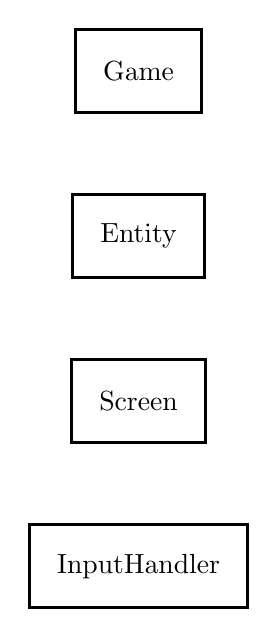
\begin{tikzpicture}[node distance=1cm, auto]  
\tikzset{
	    mynode/.style={rectangle,align=left,draw=black, top color=white, bottom color=white!50,very thick, inner sep=1em, minimum size=3em, text centered},
	    myarrow/.style={->, >=latex', shorten >=1pt, thick},
	    mylabel/.style={text width=7em, text centered} 
	}  
	\node[mynode] (game) {Game};
	\node[mynode, below=1cm of game] (entity){Entity};
	
	\node[mynode, below=1cm of entity] (screen){Screen};
	\node[mynode, below=1cm of screen] (inputhandler){InputHandler};

\end{tikzpicture} 
	\medskip

\\\\

\begin{tabularx}{\textwidth}{| p{0.7cm} | p{1.5cm} | X |}
\hline
\rowcolor[gray]{0.9} Klasse & Beschreibung
\hline
Game & Die Game-Klasse stellt im Allgemeinen das Spiel dar und funkioniert als Container für alle spielrevelanten Objekte.
\hline
Entity & Die Entity-Klasse stellt eine Spiele-Entität dar. Höchstwahrscheinlich werden später Gegner- und Spieler-Klasse von dieser erben.
\hline
Screen & Die Screen-Klasse stellt die allgemeine Klasse für die Graphische Ausgabe dar.
\hline
InputHandler & Die InputHandler-Klasse verarbeitet Spielereingaben.
\hline
\end{tabularx}